
%(BEGIN_QUESTION)
% Copyright 2015, Tony R. Kuphaldt, released under the Creative Commons Attribution License (v 1.0)
% This means you may do almost anything with this work of mine, so long as you give me proper credit

Read the ``Teaching Technical Theory'' section of Appendix D (``How to Use This Book -- Some Advice for Teachers'') in your {\it Lessons In Industrial Instrumentation} textbook.  This will serve as the basis for a discussion on why the second-year Instrumentation courses are not lecture-based.

\vskip 10pt

Imagine a child wishing to learn how to ride a bicycle.  Seeking knowledge on the subject, the child approaches an adult asking for that adult to explain how to ride a bike.  The adult responds with a detailed and thorough explanation of bicycle riding, including all the relevant safety rules.  {\it After this explanation concludes, will the child be able to ride a bicycle?}  Now imagine that same child reading a book on bicycle riding.  The book is well-written and filled with clear illustrations to aid understanding.  {\it After finishing this book, will the child be able to ride a bicycle?}  Now imagine that same child watching a demonstration video on bicycle riding.  The video is professionally shot, with very clear views on technique.  The actor in the video does a great job explaining all the important aspects of bicycle riding.  {\it After watching the video in its entirety, will the child be able to ride a bicycle?}

It should be obvious at this point that there is more to learning how to ride a bicycle than merely being shown how to do so.  Bike riding is a skill born of {\it practice}.  Instruction may be {\it necessary} to learn how to ride a bicycle safely, but instruction in itself is not {\it sufficient} to learn how to ride a bicycle safely -- you must actively attempt riding a bicycle before all the pieces of information come together such that you will be proficient.  {\it What is it about bicycle riding that necessitates \underbar{practice} in order to learn?}

\vskip 10pt

Now imagine someone wishing to learn how to write poetry.  Seeking knowledge on the subject, this person consults poets for advice, reads books of poetry and books about writing poetry, and even listens to audio recordings of poets presenting their work in public.  {\it After all this instruction and research, will the person be a proficient poet?}

Here we have the same problem we had with learning to ride a bicycle: instruction may be a {\it necessary} part of learning to write poems, but instruction in itself is not {\it sufficient} to become a poet.  One must actively write their own poems to become good at it.  {\it What is it about poetry that necessitates \underbar{practice} in order to learn how to write it?}

\vskip 10pt

The fundamental principle here is that {\it we master that which we practice}, because the brain strengthens neural pathways through repeated use.  There is nothing unique about bicycle riding or poetry in this regard: if you wish to master any skill you must repeatedly {\it do} that skill.  The problem with learning about bicycle-riding or poetry from other people is that you aren't {\it doing} any bicycle riding or poetry yourself.  The most valuable assistance any learner can receive is prompt and constructive feedback during the learner's practice.  Think of a child attempting to ride a bicycle with an adult present to observe and give practical advice; or of a person learning poetry, submitting their poems to an audience for review and then considering that feedback before writing their next poem.

When we research which skills are most valuable to instrument technicians, we find {\it self-directed learning} and {\it general problem-solving} top the list.  These skills, like any other, require intensive practice to master.  Furthermore, that practice will be optimized with prompt and expert feedback.  In order to optimally prepare students to become instrument technicians, then, those students must be challenged to learn on their own and to individually solve problems, with the instructor coaching them on both activities.

Here is where schools tend to cheat students: the majority of class time is spent presenting information to students, rather than giving students opportunity to practice their problem-solving skills.  This is primarily the consequence of {\it lecture} being the dominant mode of teaching, where a live instructor must spend hour upon hour verbally presenting information to students, leaving little or no time for those students to solve problems and sharpen their critical thinking skills.  Assigned homework does a poor job of providing practice because the student doesn't receive detailed feedback on their problem-solving strategies, and also because many students cheat themselves by receiving inappropriate help from their classmates.  Furthermore, lecture is the antithesis of self-directed learning, being entirely directed by a subject matter expert.  The skills practiced by students during a lecture (e.g. taking dictation on lengthy presentations) have little value in the career of an instrument technician.  More time in school could be spent practicing more relevant skills, but only if some other mode of instruction replaces lecture.

\vfil \eject

\noindent
Not only does lecture displace more valuable activities in the classroom, but lecture isn't even that good of an instructional technique.  Among the serious shortcomings of lecture are the following:

\begin{itemize}
\item{} Students' attentions tend to drift over the span of any lecture of significant length.
\vskip 5pt
\item{} Lecture works well to communicate facts and procedures but fails at getting students to think for themselves, because the focus and pace of any lecture is set by the lecturer and not the students.
\vskip 5pt
\item{} Lecture instills a false sense of confidence in students, because complex tasks always look easier than they are when you watch an expert do it without trying it yourself.  (An oft-heard quote from students in lecture-based classes: {\it ``I understand things perfectly during lecture, but for some reason I just can't seem to do the homework on my own!''})
\vskip 5pt
\item{} A lecturer cannot customize (``differentiate'') instruction for individual students.  Rather, everyone gets the exact same presentation (e.g. the same examples, the same pace) regardless of their diverse needs.  The pace of lecture is perhaps the most obvious example of this problem: since the lecturer can only present at one pace, he or she is guaranteed to bore some students by going to slow for them and/or lose others by going too fast for them.
\vskip 5pt
\item{} Students cannot ``rewind'' a portion of lecture they would like to have repeated without asking the entire class to repeat as well.
\vskip 5pt
\item{} Students' must simultaneously dictate notes while trying to watch {\it and} listen {\it and} think along with the instructor, a difficult task at best.  Multitasking is possible only for simple tasks, none of them requiring intense focus.
\vskip 5pt
\item{} If the instructor commits some form of verbal error and doesn't realize it (which is very common because it's difficult to simultaneously present and self-evaluate), it is incumbent upon the students to identify the error and ask for clarification.
\vskip 5pt
\item{} The instructor cannot accurately perceive how each and every student is understanding the presentation, because the instructor is too busy presenting.  Body language during the lecture isn't a reliable enough indicator of student understanding, and the time taken by lecture precludes the instructor visiting every student to inspect their work.
\vskip 5pt
\item{} Lecture instills an attitude of dependence on students by reinforcing the notion they need to personally consult an expert in order to learn anything new.  This discourages students from even trying to learn complex things on their own.
\end{itemize}

\vskip 10pt

For these reasons -- the fact that lecture displaces class time better spent coaching students to solve problems, as well as the many problems of lecture as an instructional mode -- there is almost no lecture in any of the 200-level Instrumentation courses at BTC.  Instead, students learn the basic facts and procedures of the subject matter through reading assignments prior to class, then spend class time solving problems and demonstrating their understanding of each day's major topic(s) before leaving.  This is called an {\it inverted classroom} because the classroom and homework roles are swapped: what is traditionally lectured on in class is instead done on the students' time outside of class, while the problem-solving traditionally done as homework is instead completed during class time while the instructor is available to coach.  This format is highly effective not only for learning the basic concepts of instrumentation, but also for improving technical reading and critical thinking skills, simply because {\it it requires students to practice the precise skills they must master}.

The primary reason {\it reading} was chosen as the preferred mode of instruction is feedback from employers as well as observations of student behavior, both sources revealing an aversion to technical reading.  Some employers (most notably the BP oil refinery in Carson, California) noted reading comprehension as being the weakest area when testing BTC students during recruiting trips.  Also, a failure to reference equipment manuals when working on real systems is a chronic problem both for novice technicians in a wide range of industries as well as students learning in a lab environment.  Given the fact that far more high-quality technical information is available for continued learning in this career than high-quality videos, reading comprehension is a vital skill for technicians to keep their knowledge up to date as technology advances.

\vfil \eject

Prior to 2006 all 200-level Instrumentation courses were strictly taught by lecture.  Making matters worse, many of the courses had no textbook, and homework was seldom assigned.  All 200-level exams prioritized rote memorization and execution of procedural problem-solving over creative problem-solving and synthesis of multiple concepts.  It was common for second-year students to flounder when presented with a new piece of equipment or a new type of problem, because no instructor can teach procedures to cover any and all possible challenges.

\vskip 10pt

Since 2006 the 200-level Instrumentation courses have gradually morphed from lecture to ``inverted'' format, with measurable gains in learning.  Proportional exam scores from the Fall quarter courses (INST240, INST241, and INST242 -- those courses where the content has remained most stable over this time span) demonstrate this, each histogram showing the number of students (vertical axis) achieving a certain exam score (horizontal axis):

$$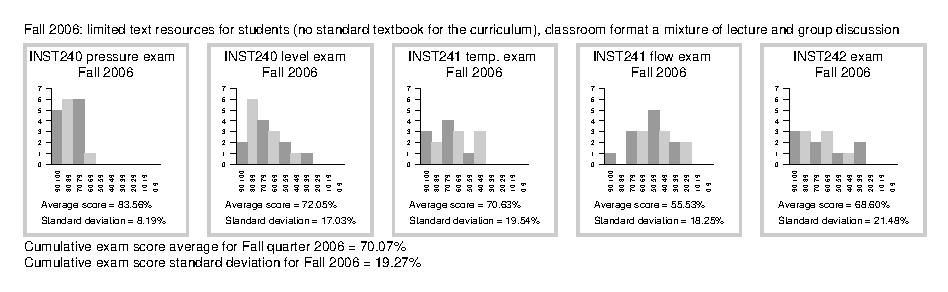
\includegraphics[width=15.5cm]{i00004x01.eps}$$

$$\includegraphics[width=15.5cm]{i00004x02.eps}$$

$$\includegraphics[width=15.5cm]{i00004x03.eps}$$

Note the general improvement in average exam scores (2009) toward the end of the quarter, despite the exams being more complex than they were in 2006.  Students were held accountable for the assigned textbook reading with graded ``prep quizzes'' at the beginning of each class session.  Note also how the standard deviations increased, representing a greater degree of ``spread'' between student performance on these exams.  The increased standard deviation shows some students falling behind their peers, since lecture was not providing for their needs with a more challenging curriculum.

In the third set of histograms (2013) we see general increases in average scores as well as marked improvements in standard deviation across the board (showing fewer students ``left behind'' their peers).  The inverted classroom format allows the instructor to spend one-on-one time with each and every student to probe for misconceptions and offer assistance when needed.  This kind of differentiated instruction is impossible in a lecture format.  Even more remarkable is the fact that the exam complexity increased since 2009, with longer mastery exams (reviewing concepts from previous courses including first-year circuit principles) and more complex proportional exams.  In 2013 the exams so fully exhausted the 3-hour testing period that graded results could no longer be given before the end of the day, and instead had to wait until the following day.  Yet, despite this increased rigor exam scores increased and standard deviation narrowed.

%\vfil \eject

\vskip 10pt

One of the most striking improvements realized since abandoning lecture is the ease of which students grasp some of the more complex concepts throughout the year.  These concepts used to be difficult to convey in a lecture format (mostly due to pacing problems, since different students would get ``stuck'' at different points in the presentation), and so long as some lecture existed in the classroom students would tend to give up when they encountered difficult concepts in the assigned reading (knowing they could rely on the instructor to lecture on these tough concepts in class):

\begin{itemize}
\item{} INST230 course: Three-phase electric power system calculations
\item{} INST230 course: Normally-open versus normally-closed contact status
\item{} INST240 course: Interface liquid level measurement (hydrostatic and displacer)
\item{} INST240/250 courses: Force-balance versus motion-balance pneumatic mechanisms
\item{} INST241 course: Coriolis mass flowmeters
\item{} INST242 course: Gas chromatograph operation
\begin{itemize}

\end{itemize}
\item{} INST242 course: Non-dispersive optical analyzers (NDIR, Luft detectors, etc.)
\begin{itemize}

\end{itemize}
\item{} INST250 course: Fluid power system analysis (hydraulic and pneumatic diagrams)
\item{} INST250 course: Split-ranged control valve sequencing
\item{} INST250 course: Control valve characterization
\begin{itemize}

\end{itemize}
\item{} INST252/263 courses: Feedforward control strategies
\begin{itemize}

\end{itemize}
\item{} INST252 course: Loop stability analysis (based on trend recordings)
\item{} INST260 course: Data acquisition hardware connections (e.g. differential vs. single-ended connections)
\item{} INST262 course: FOUNDATION Fieldbus and wireless (radio) digital communications
\begin{itemize}

\end{itemize}
\item{} INST263 course: Selector and override controls
\end{itemize}

This improvement in student learning has been verified by industry representatives, when they are invited to come to BTC to review certain complex topics such as Fieldbus, WirelessHART, and control valves.  The general feedback they give is that BTC students are unusually well-prepared on these subjects.  The ``secret'' of course is that students learning in an inverted classroom format spend more time immersed in the subject matter, and the feedback they receive from their instructors in class is better tailored to their individual learning needs.

\vskip 10pt

Another significant gain realized since abandoning lecture is the immediate placement of inexperienced BTC Instrumentation graduates in jobs typically reserved for engineers with 4-year degrees.  This simply did not happen when BTC's Instrumentation program was lecture-based, and it is due to the fact that students explicitly learn higher-order thinking skills when they must gather information on their own outside of class and then demonstrate critical thinking before an instructor every day.  This has happened once in December 2011, again in December 2012, again in March 2013, and again in August 2013.

\vskip 20pt

Yet, despite the gains realized by abandoning lecture in favor of an ``inverted'' teaching format, some students are highly resistant to the concept.  Some of the critical comments routinely heard from students against the inverted format are as follows:

\begin{itemize}
\item{$(1)$} {\it ``I learn better in a lecture format.''}
\vskip 5pt
\item{$(2)$} {\it ``My learning style is visual, which means I need to \underbar{see} someone solve the problems for me.''}
\vskip 5pt
\item{$(3)$} {\it ``When I arrive to class after doing the assigned reading and trying to solve the homework problems, I'm completely lost.''}
\end{itemize}

\vskip 10pt

Discuss each of these comments in detail.  Here are some starting points for conversation:

\begin{itemize}
\item{$(1)$} What does it mean to learn something {\it better}?  How may a student measure how well they've learned something new?  What, exactly, is it that is learned better in lecture?  Is there anything significant that students {\it don't} learn in a lecture?
\vskip 5pt
\item{$(2)$} Would someone with an {\it auditory} or {\it kinesthetic} learning style fare any better in an inverted classroom?  Does a visual learning style preclude effective reading, or independent learning?  Are learning styles real or merely perceived?  Are learning styles immutable (i.e. permanent), or is it possible for people to cultivate new learning styles?
\vskip 5pt
\item{$(3)$} What does it mean if a student is lost after completing the homework for an inverted class, assuming a significant number of their classmates are {\it not} lost?  What would be an appropriate course of action to take in response to this condition?
\end{itemize}

\vskip 10pt

\underbar{file i00004}
%(END_QUESTION)





%(BEGIN_ANSWER)


%(END_ANSWER)





%(BEGIN_NOTES)

Here is a timeline for the transition away from lecture and toward an inverted classroom in the second-year (200-level) Instrumentation courses:

\begin{itemize}
\item{} {\bf October 1998:} Hired to teach first year of Instrumentation at BTC.  Surveying student comments, I heard a lot of things like {\it ``High school was more challenging than this!''}  Some students flatly rejected by employers ({\it ``Don't ever send us anyone like that again''} was one comment heard by a supervisor at the BP Cherry Point refinery following a jobshadow).  No lesson plans existed for anything taught in the first or second years of the program.
\vskip 10pt
\item{} {\bf 1998-1999:} My first year of teaching, like every teacher's first year of teaching, was very rough.  At times I felt like I was barely discharging the duties of my job, all the required tasks were so overwhelming.
\vskip 10pt
\item{} {\bf 1999-2000:} Developed lessons plans for each day of teaching, including live demonstrations of concepts for most every day.
\vskip 10pt
\item{} {\bf 1998-2001:} Most common student complaint: {\it ``I understand things perfectly when you explain them to me, but for some reason I just can't seem to do it on my own!''}  Many students exhibiting poor recall of important concepts, even students who were clearly paying attention and doing the homework.  I was beginning to feel frustrated and even burnt out trying my best to get students to really understand electronics while seeing mediocre results.
\vskip 10pt
\item{} {\bf 2000-2001:} Overheard a conversation between two students: {\it ``This class is great -- Tony presents everything so well, you don't even have to read the book!''}  This revelation was key to cracking the problem: all the work I had put in to making polished presentations for my students was actually hurting their development as learners.  Students were coming to class expecting ``The Tony Show'' rather than preparing on their own, and this explained much of their poor retention and mastery of concepts.  The bottom line is this: {\it student learning is directly proportional to student effort,} all other factors being equal.
\vskip 10pt
\item{} {\bf December 2001:} Instrumentation advisory committee meeting, where Sam Bryant contributed his thoughts that the most important things for success in this field were \underbar{self-direction} and the \underbar{ability to independently learn}.  These things are more important than subject-matter knowledge and skill, because they enable continuous learning and advancement throughout one's career.
\vskip 10pt
\item{} {\bf January 2002-June 2002:} Met with Ed Fournier and other BTC Nursing program instructors to learn how their small-group teaching method worked.  Nursing students were assigned lists of objectives and reading assignments; they met in small groups to discuss what they learned and get clarification from instructor.  I observed several Nursing class sessions where I was astounded by the depth of engagement and understanding demonstrated by the students: it was everything I wanted to have happen in my class, but wasn't happening.  Nursing faculty warned me, however, that this was not well-received by all students -- in fact, some of them absolutely hated the process.  I encountered one of these frustrated students working as a cashier at Fred Meyer, who told me in no uncertain terms, {\it ``I learn better in lecture!''}
\vskip 10pt
\item{} {\bf 2002-2003:} Taught second year of program for the first time, in parallel with another instructor.  This was my first time implementing ``research-discussion'' rather than lecture-based teaching.  Students initially revolted: {\it ``If I'd wanted to study, I would have gone to a real college!''} but I pushed back and they eventually came around to liking the format.  In the end, it worked phenomenally well, with my student group out-performing the lecture-taught group in every metric (handling more advanced test questions and more advanced lab projects, and using less time in class).  Used B\'ela Lipt\'ak's {\it Instrument Engineers Handbook} series as our text, because I couldn't find anything else suitable.
\vskip 10pt
\item{} {\bf 2003-2004:} First year of program taught by another instructor (Larry), who tried applying the research-discussion method.  Half of his class revolted as well, even involving a counselor in the fight.  During a whole-class discussion moderated by the counselor, one of the harder-working students (who was Ukrainian) stood up and angrily denounced those opposing students as ``Lazy Americans'' ({\it ``In Ukraine, we write notes in margins of newspaper, we were so poor!  Here you have everything you need to learn, but you don't do the work!!''}).  In the end this instructor capitulated to the complaints and returned to lecture, but regretted doing so.
\vskip 10pt
\item{} {\bf 2004-2005:} Moved to DMC building, implemented new first-year curriculum based on research and discussion.
\vskip 10pt
\item{} {\bf 2005-2006:} Continued teaching with inverted classroom structure.  Problems noted in student preparation: no matter how often I encouraged students to do their homework, many of them only invested a cursory effort.  This was also noted by the harder-working students, who complained about peers not coming to class prepared.
\vskip 10pt
\item{} {\bf June 2006:} The 2nd-year instructor left BTC to take position in industry.
\vskip 10pt
\item{} {\bf 2006-2007:} Taught 2nd year of program, using a completely rewritten curriculum based on lessons learned.  Student preparation still judged via inspection of homework notes, although this was proving to be problematic.  One class discussion highlighted this problem, with the harder-working students complaining that many of their peers didn't even bother to do their homework ahead of class.  When one of those ill-prepared students countered with a complaint about having to read too much, another student replied that anyone who couldn't learn by reading {\it ``. . . is profoundly disadvantaged in an information-based society!''}
\vskip 10pt
\item{} {\bf 2007-2008:} Incorporated daily quizzes into grading, rather than homework inspection.
\vskip 10pt
\item{} {\bf Summer 2008:} Began writing {\it Lessons In Industrial Instrumentation} due to a total lack of suitable instrumentation textbooks on the market.
\vskip 10pt
\item{} {\bf 2008-2009:} Marked improvements in student comprehension with the new textbook available as a learning resource.
\vskip 10pt
\item{} {\bf April-June 2009:} Some students still arriving in class wholly unprepared (didn't do homework), with no change in behavior after repeated counsel.  Announcement made regarding change to quiz grading prior to summer break.
\vskip 10pt
\item{} {\bf September 2009:} Prep/summary quiz grading changed to -1\% per failed quiz.
\vskip 10pt
\item{} {\bf November 2009:} One student (who was notorious in his lack of preparation) filed a grievance against me regarding the new quiz policy.  Met with Dean in January of 2010, and emerged from that meeting with the new quiz policy still intact.  One of the lines of evidence used to uphold the new quiz grading policy is that the mastery exam failure rate was cut in half immediately following the change!
\vskip 10pt
\item{} {\bf 2009:} Added circuit fault analysis question (i.e. choosing ``Possible'' or ``Impossible'' for proposed faults in a malfunctioning circuit) to all mastery exams.
\vskip 10pt
\item{} {\bf 2010-2011:} Whole-class Socratic discussions abandoned in favor of small-group interactions.  One of the major motivations for this was the increase in class size (40 students total), which made it difficult for students to hear each other in an auditorium-style classroom.
\vskip 10pt
\item{} {\bf 2010-2011:} Tried holding question \& answer sessions at the very beginning of class, to address student complaints about having to pass quizzes after only having studied the material on their own.  What resulted from this experiment was sobering: only two students ever asked questions during these sessions.  The rest of them either had no need for the Q\&A session or they had cut back on their preparation because they knew I would be explaining the more challenging concepts at the start of class.
\vskip 10pt
\item{} {\bf August 2011:} Received a telephone call from an employer about a graduate who was doing very poorly at his job.  This particular job required that the graduate learn how to use a specific software application.  He was having trouble learning the features of this program.  The employer told me she had recommended this grad take notes on how to use this software, documenting each new thing he learned, as a way to teach himself, but that the grad refused to do this and so was floundering in his job.  Not surprisingly, this grad exhibited a severe deficit in self-motivation in class, barely passing many of the second-year courses.  On a side note, he was really personable and easy to work with, but clearly did not take responsibility for his learning.
\vskip 10pt
\item{} {\bf September 2011:} Abandoned Q\&A at the start of class, due to abuse.  The same few students were the only people who ever asked questions, with many others neglecting to do their homework because they figured they could just learn the day's topics from these Q\&A sessions.
\vskip 10pt
\item{} {\bf 2014:} Added third review question to all mastery exams, such that every mastery exam now reviews important concepts from {\it every} previous quarter in the second year of the program.
\vskip 10pt
\item{} {\bf April 2014:} Added DC/AC circuit analysis review question (i.e. applying fundamental analysis principles such as Kirchhoff's Laws and transformer ratios to simple circuits) to all mastery exams.
\vskip 10pt
\item{} {\bf May 2015:} Upon learning that our traditional 3-hour classroom block schedules would likely disappear in favor of shorter class sessions campus-wide (1 hour, 20 minutes each) for room-scheduling efficiency, Bobby and I experimented with a new theory session format.  Small groups of students (no more than four to a group) would sign up for half-hour timeslots to check off their homework with either Bobby or myself in our lab room rather than the classroom.  This took place between Noon and 3 PM (still a three-hour block) but we no longer needed to use the classroom and students had more freedom in how they spent their time.  This also makes it possible to teach other courses to small groups of students during unallocated half-hour timeslots (e.g. elective courses for non-Instrumentation students).  Direct inspection of homework replaced the customary ``prep quiz'' while the rest of the check-off process continued as usual, answering student questions and challenging students to answer new questions.  Any students not strong on any concept at the end of the half-hour session were given half-credit if they could come back later that day demonstrating a strong understanding of the concept(s).  Test scores comparable with previous years, less stress during checkoffs due to lower noise levels, seemingly greater detail in student note-taking (outlines of reading).  Mastery exam re-takes done in the afternoon (rather than during lab time), outside of each student's designated time slot.
\vskip 10pt
\item{} {\bf LESSONS LEARNED:} Student achievement is a direct function of student effort.  The biggest impediment to student learning by far is students' own reluctance to study independently.  The biggest challenge for me as an instructor is how to overcome the cultural bias created by years of compulsory education where shallow, lecture-based instruction is the norm; where teachers spoon-feed information to students; where exams may be passed by doing nothing more than recalling definitions and executing memorized procedures.  General reluctance to study hard is not a mark of individual laziness.  If it were, only a minority of students would exhibit this behavior.
\end{itemize}



%INDEX% Course organization, inverted classroom

%(END_NOTES)


